\part{Entrega 2}

\section{Introducción}

En este informe, se llevará a cabo un análisis estructural de un enrejado de la entrega 1, considerando la sección transversal más grande estudiada (\(A_{30}\)). Se evaluarán dos configuraciones posibles para el enrejado: una con una diagonal en cada cara y otra con dos diagonales cruzadas en las caras laterales e interiores. El objetivo es analizar cómo las deformaciones y las fuerzas axiales de las barras se comportan bajo diferentes condiciones de carga, específicamente con una aceleración de 0.1g en los tres ejes y un aumento de temperatura de 100°C en los nodos.

El análisis se dividirá en dos partes. En la primera, se analizarán las deformaciones y las fuerzas axiales en función de las condiciones de aceleración y temperatura, mostrando las deformaciones y la distribución de las fuerzas axiales para cada caso. En la segunda parte, se estudiará la "peor dirección" de aceleración, entendida como la dirección en la que se maximiza o minimiza la carga axial en las barras, considerando que la aceleración puede ser en cualquier dirección en el espacio 3D.

\section{Resultados}

\subsection{Parte 1}

Para esta sección se seleccionó un reticulado de 16 vanos para una mejor visualización de los resultados. A este, se le realizaron análisis de deformación y esfuerzos internos frente a aceleraciones aplicadas en cada dirección $x$, $y$, $z$. Posteriormente, se compararon y obtuvieron los resultados pertinentes.

\subsubsection{Aceleración en Eje X}

\begin{figure}[H]
    \centering
    \begin{minipage}{0.45\textwidth}
        \centering
        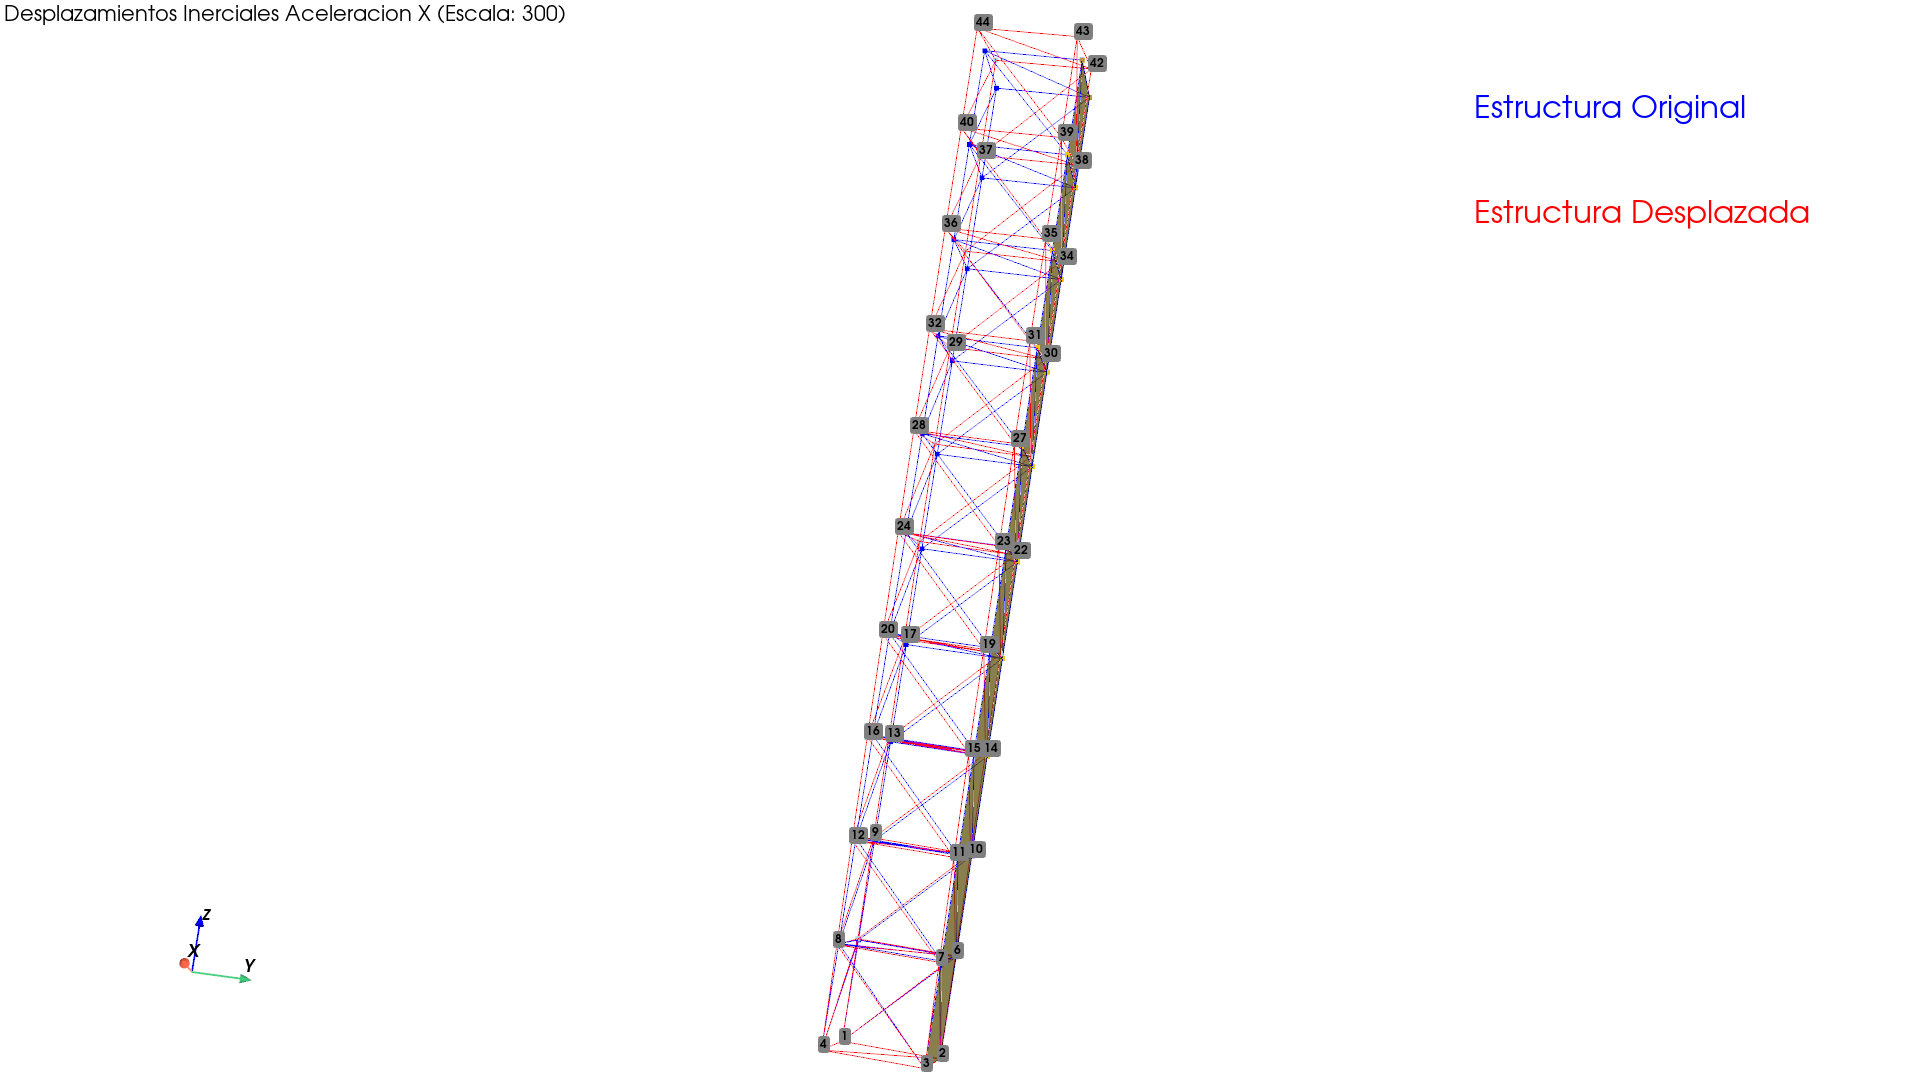
\includegraphics[width=\textwidth]{GRAFICOS/Desplazamientos Inerciales Aceleracion X False.png}
        \caption{Desplazamiento en X estructura sin diagonales cruzadas.}
        \label{fig:imagen1}
    \end{minipage}
    \hfill
    \begin{minipage}{0.45\textwidth}
        \centering
        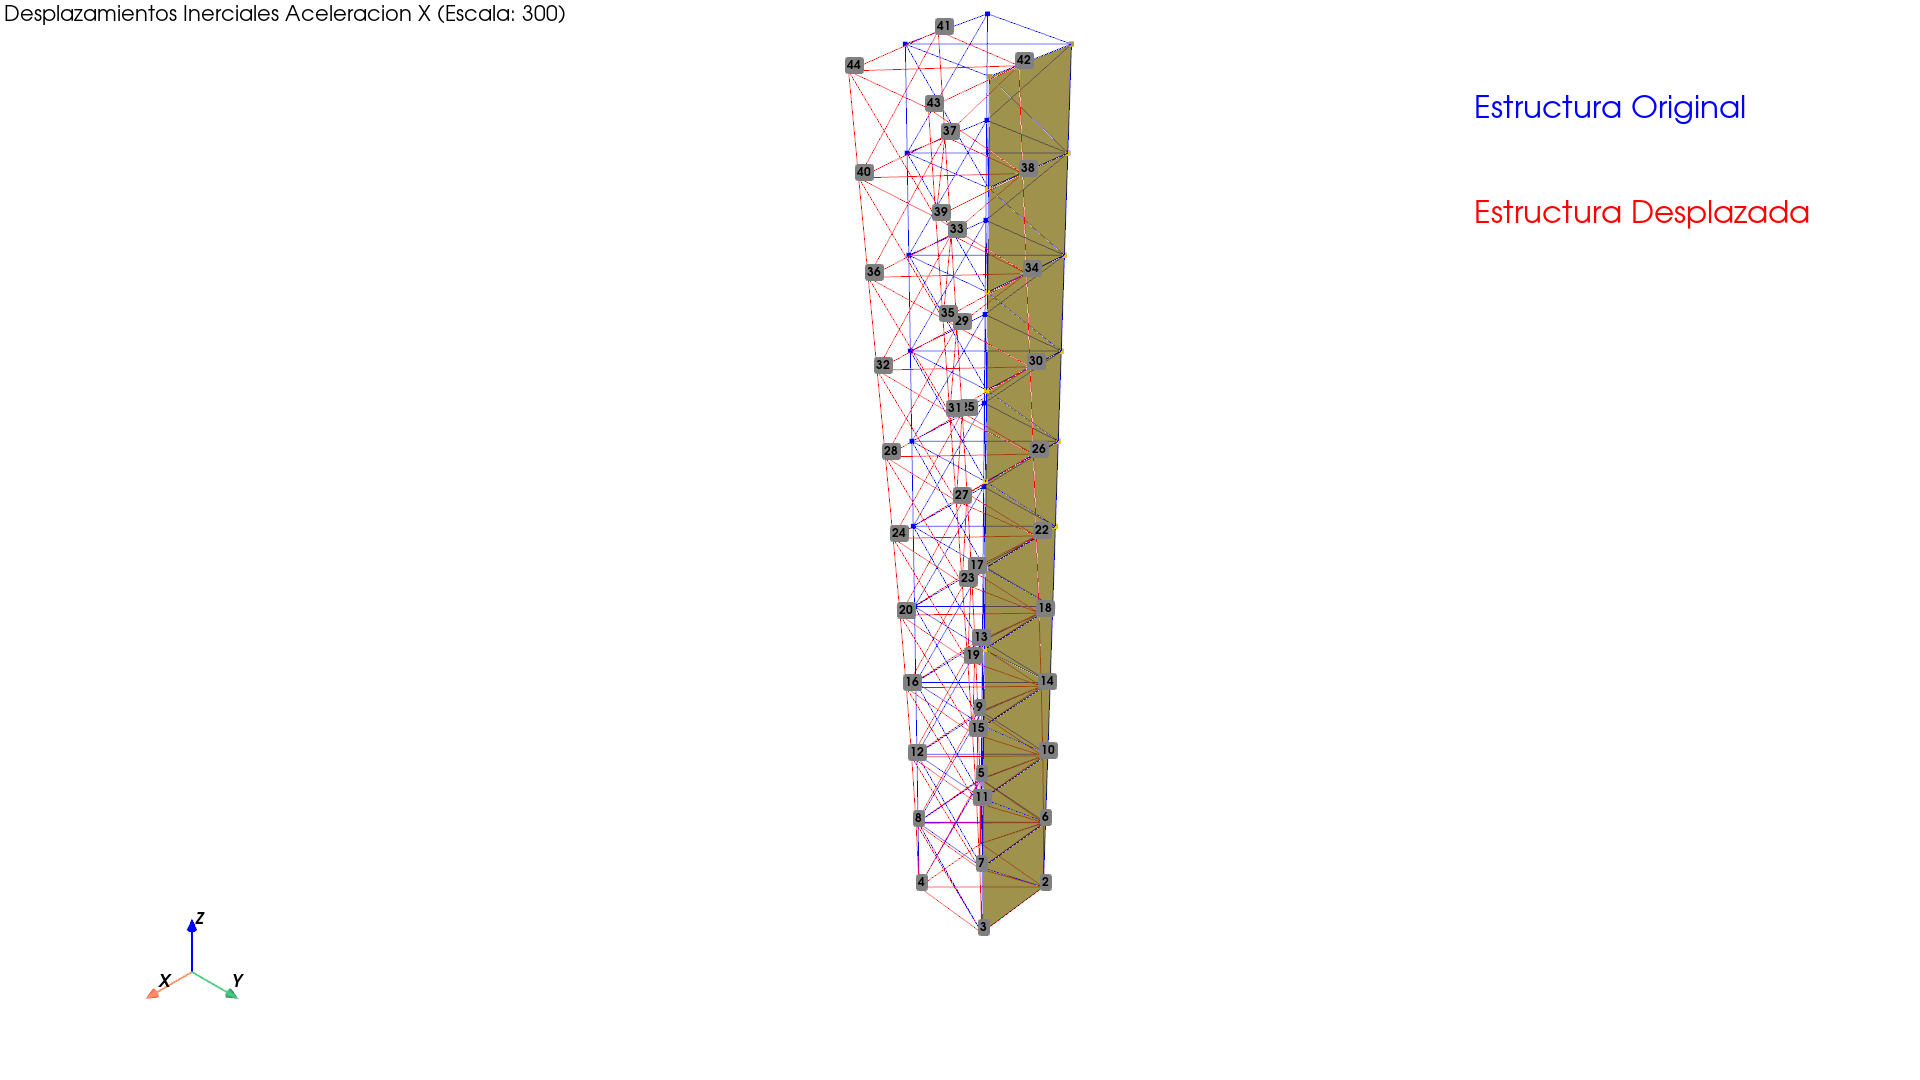
\includegraphics[width=\textwidth]{GRAFICOS/Desplazamientos Inerciales Aceleracion X True.png}
        \caption{Desplazamiento en X estructura con diagonales cruzadas.}
        \label{fig:imagen2}
    \end{minipage}
\end{figure}

\begin{figure}[H]
    \centering
    \begin{minipage}{0.45\textwidth}
        \centering
        \includegraphics[width=\textwidth]{GRAFICOS/Esfuerzos Internos Máximos en las Barras Aceleracion X False.png}
        \caption{Esfuerzos internos en estructura sin diagonales cruzadas.}
        \label{fig:imagen11}
    \end{minipage}
    \hfill
    \begin{minipage}{0.45\textwidth}
        \centering
        \includegraphics[width=\textwidth]{GRAFICOS/Esfuerzos Internos Máximos en las Barras Aceleracion X True.png}
        \caption{Esfuerzos internos en estructura con diagonales cruzadas.}
        \label{fig:imagen22}
    \end{minipage}
\end{figure}

\subsubsection{Aceleración en Eje Y}

\begin{figure}[H]
    \centering
    \begin{minipage}{0.45\textwidth}
        \centering
        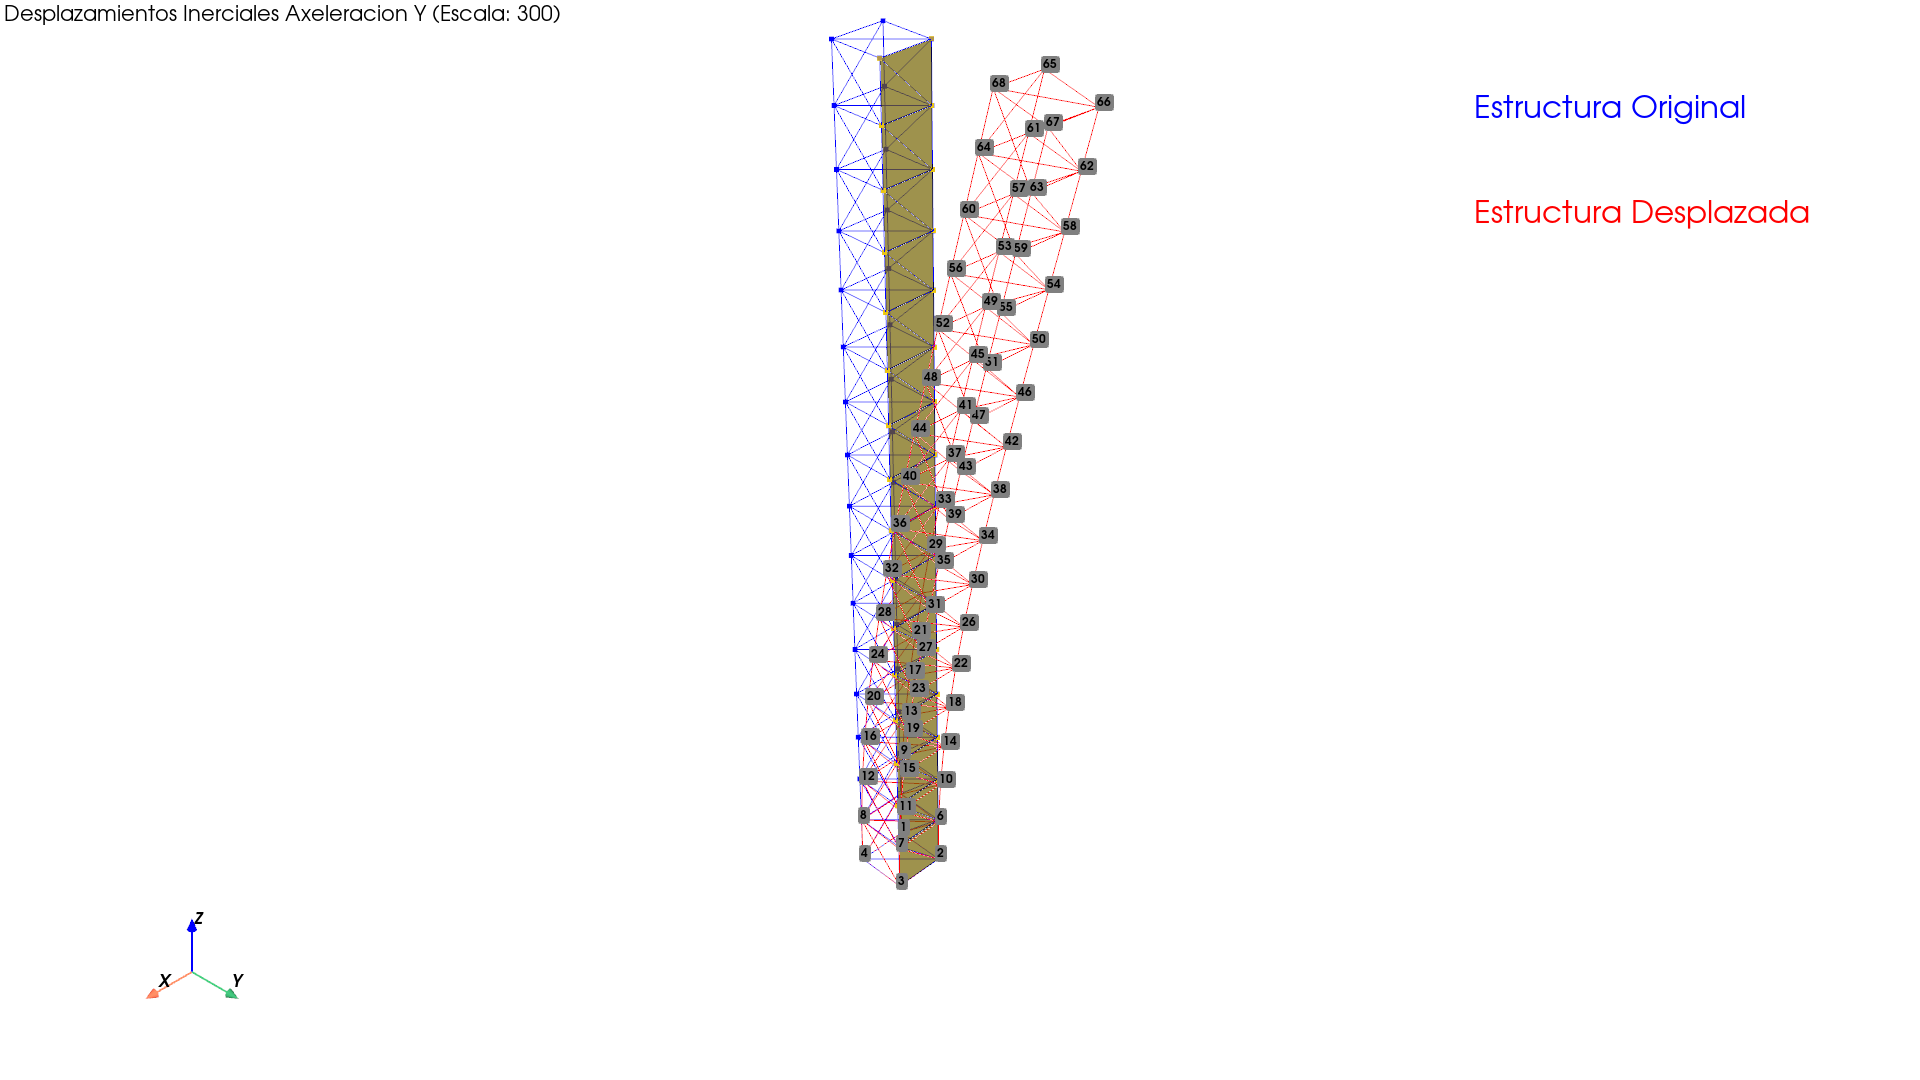
\includegraphics[width=\textwidth]{GRAFICOS/Desplazamientos Inerciales Axeleracion Y False.png}
        \caption{Desplazamiento en Y estructura sin diagonales cruzadas.}
        \label{fig:imagen3}
    \end{minipage}
    \hfill
    \begin{minipage}{0.45\textwidth}
        \centering
        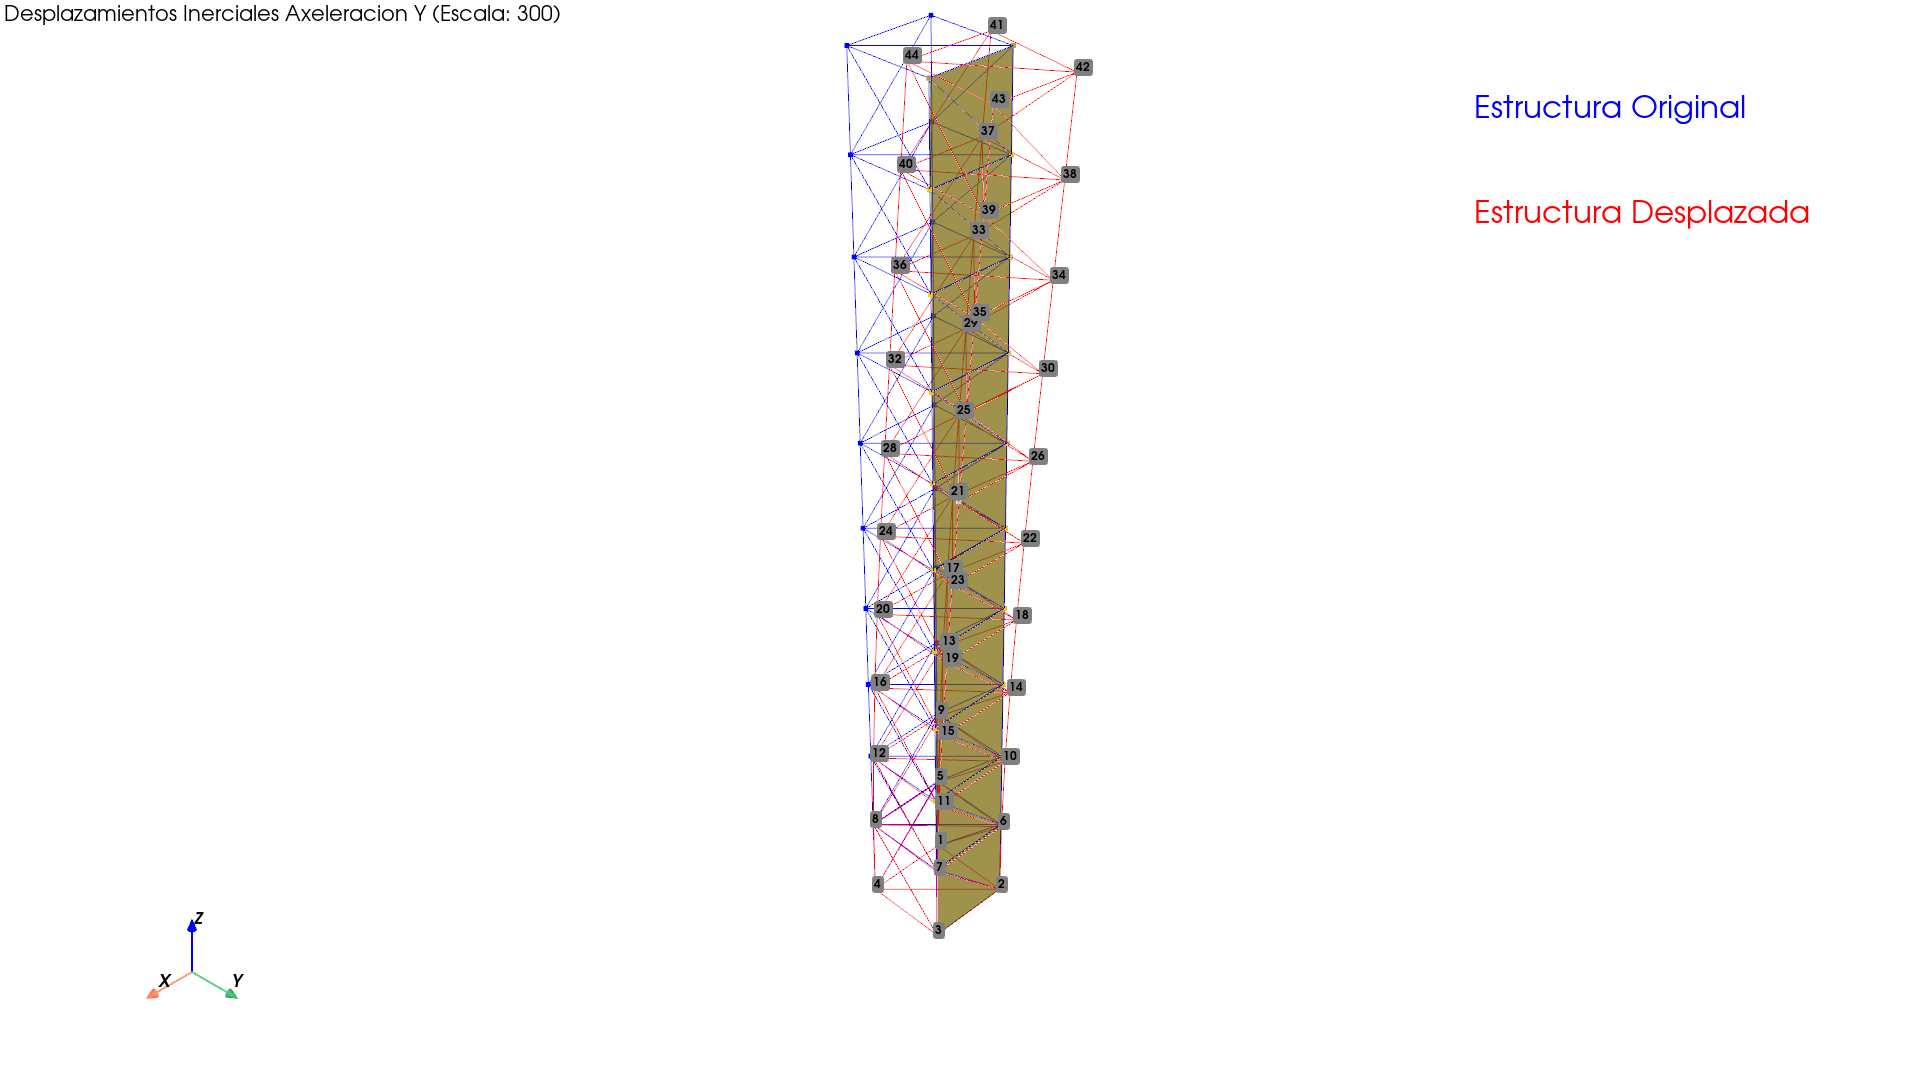
\includegraphics[width=\textwidth]{GRAFICOS/Desplazamientos Inerciales Axeleracion Y True.png}
        \caption{Desplazamiento en Y estructura con diagonales cruzadas.}
        \label{fig:imagen4}
    \end{minipage}
\end{figure}

\begin{figure}[H]
    \centering
    \begin{minipage}{0.45\textwidth}
        \centering
        \includegraphics[width=\textwidth]{GRAFICOS/Esfuerzos Internos Máximos en las Barras Axeleracion Y False.png}
        \caption{Esfuerzos internos en estructura sin diagonales cruzadas.}
        \label{fig:imagen33}
    \end{minipage}
    \hfill
    \begin{minipage}{0.45\textwidth}
        \centering
        \includegraphics[width=\textwidth]{GRAFICOS/Esfuerzos Internos Máximos en las Barras Axeleracion Y True.png}
        \caption{Esfuerzos internos en estructura con diagonales cruzadas.}
        \label{fig:imagen44}
    \end{minipage}
\end{figure}

\subsubsection{Aceleración en Eje Z}

\begin{figure}[H]
    \centering
    \begin{minipage}{0.45\textwidth}
        \centering
        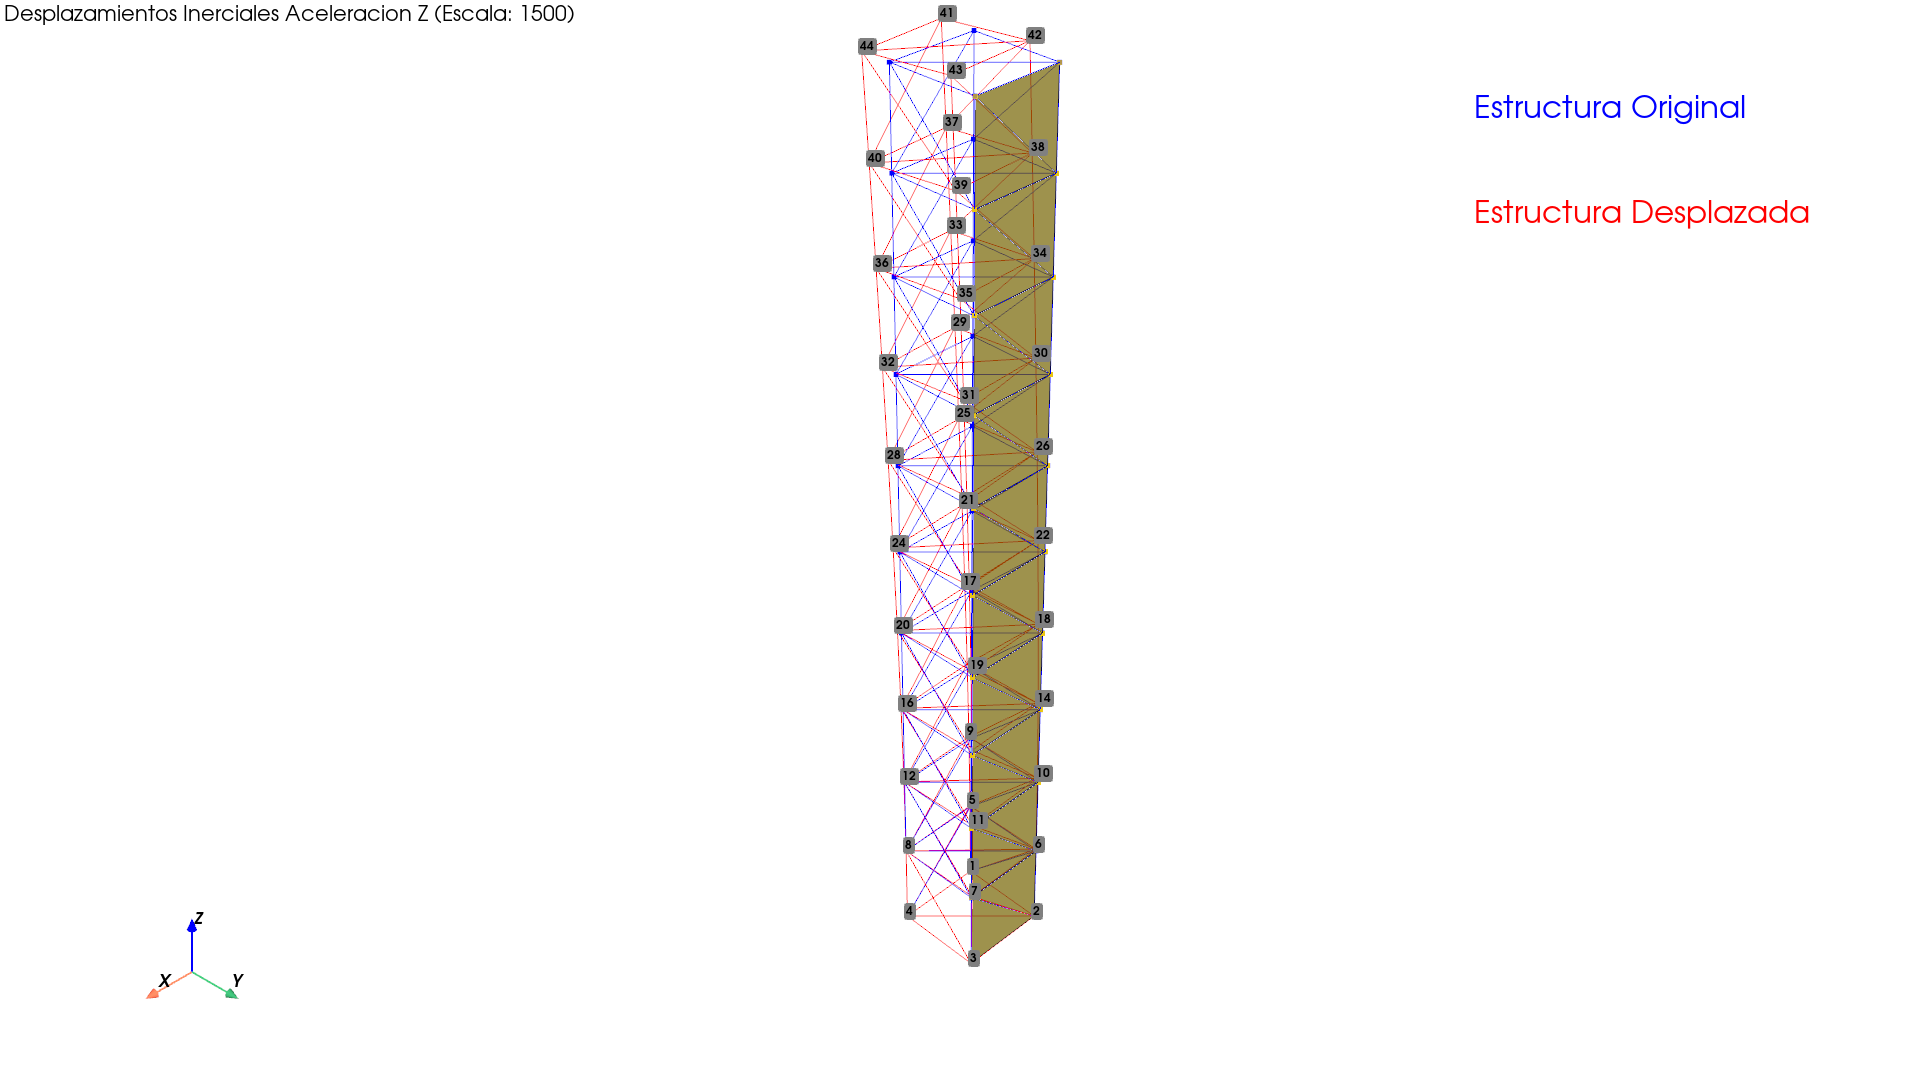
\includegraphics[width=\textwidth]{GRAFICOS/Desplazamientos Inerciales Aceleracion Z False.png}
        \caption{Desplazamiento en Z estructura sin diagonales cruzadas.}
        \label{fig:imagen5}
    \end{minipage}
    \hfill
    \begin{minipage}{0.45\textwidth}
        \centering
        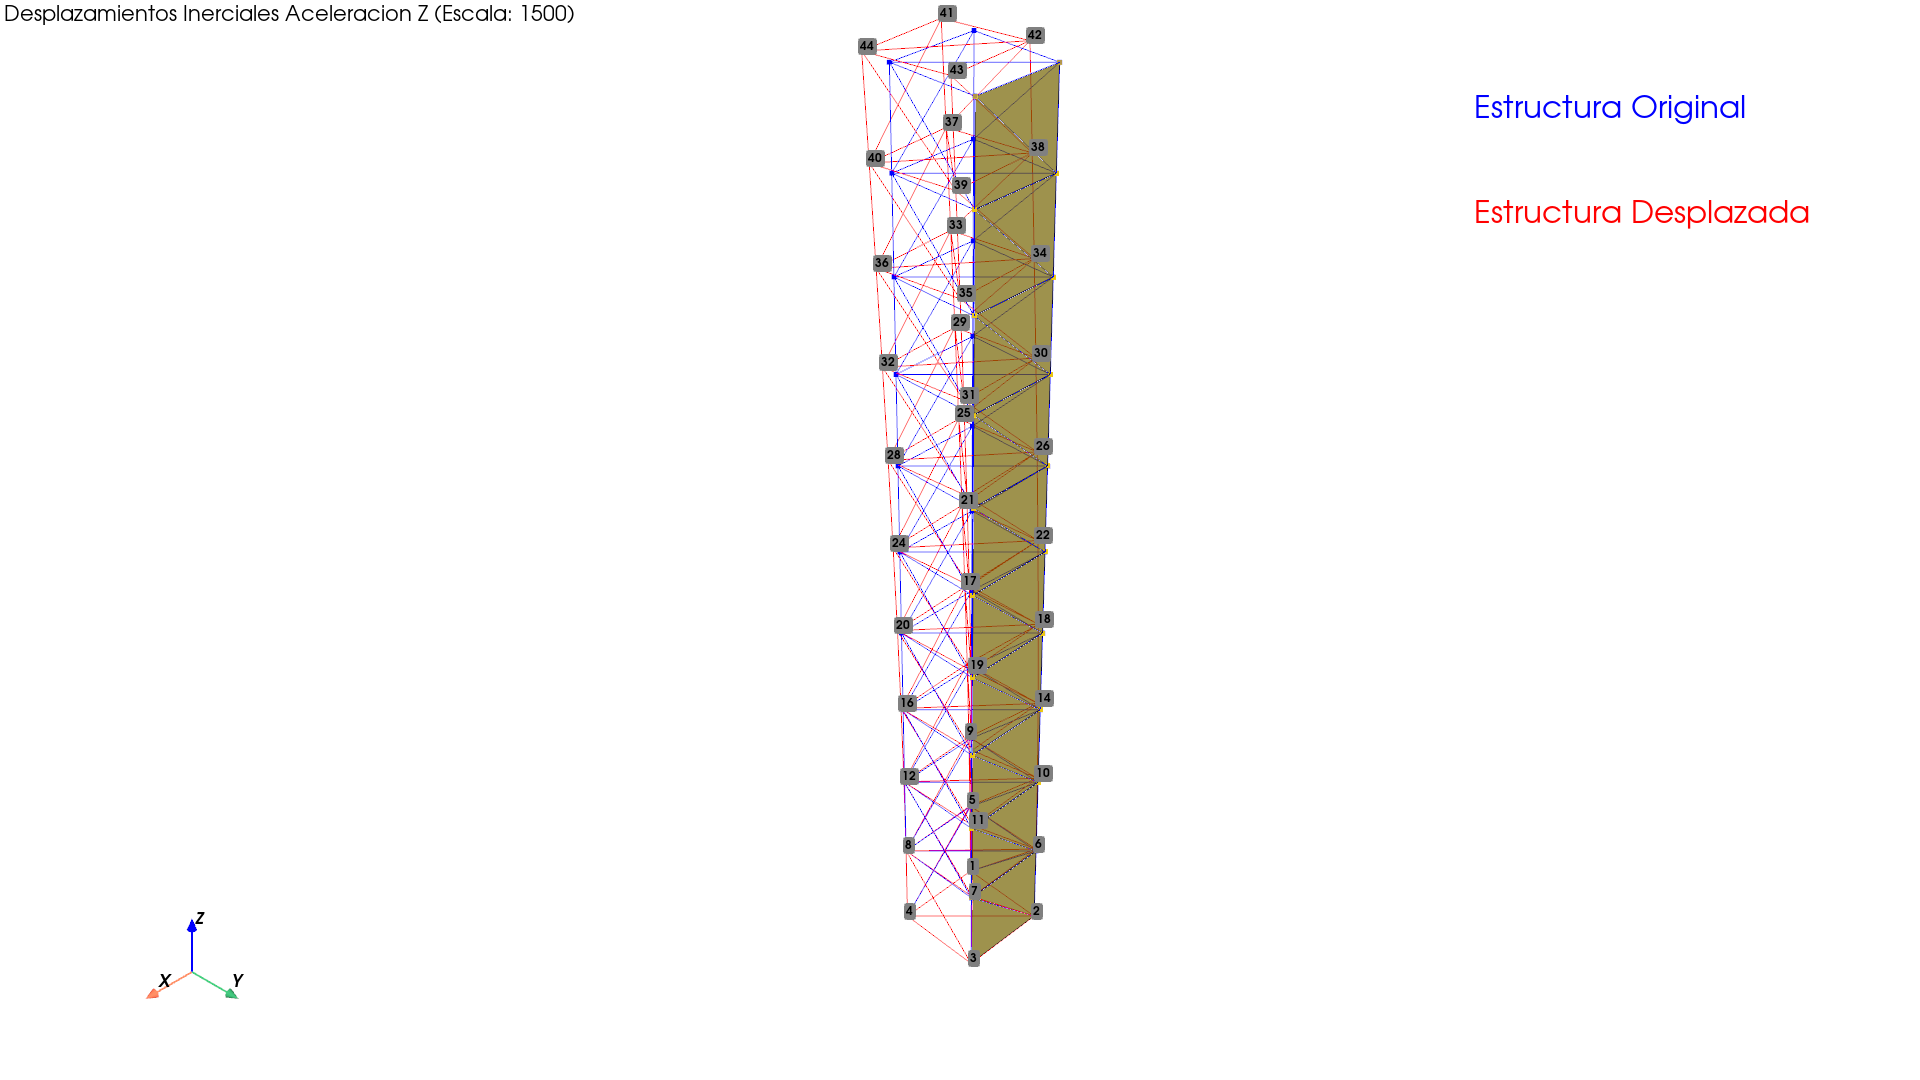
\includegraphics[width=\textwidth]{GRAFICOS/Desplazamientos Inerciales Aceleracion Z True.png}
        \caption{Desplazamiento en Z estructura con diagonales cruzadas.}
        \label{fig:imagen6}
    \end{minipage}
\end{figure}

\begin{figure}[H]
    \centering
    \begin{minipage}{0.45\textwidth}
        \centering
        \includegraphics[width=\textwidth]{GRAFICOS/Esfuerzos Internos Máximos en las Barras Aceleracion Z False.png}
        \caption{Esfuerzos internos en estructura sin diagonales cruzadas.}
        \label{fig:imagen55}
    \end{minipage}
    \hfill
    \begin{minipage}{0.45\textwidth}
        \centering
        \includegraphics[width=\textwidth]{GRAFICOS/Esfuerzos Internos Máximos en las Barras Aceleracion Z True.png}
        \caption{Esfuerzos internos en estructura con diagonales cruzadas.}
        \label{fig:imagen66}
    \end{minipage}
\end{figure}

\subsubsection{Aumento de temperatura en 100°C en nodos conectados al panel}

\begin{figure}[H]
    \centering
    \begin{minipage}{0.45\textwidth}
        \centering
        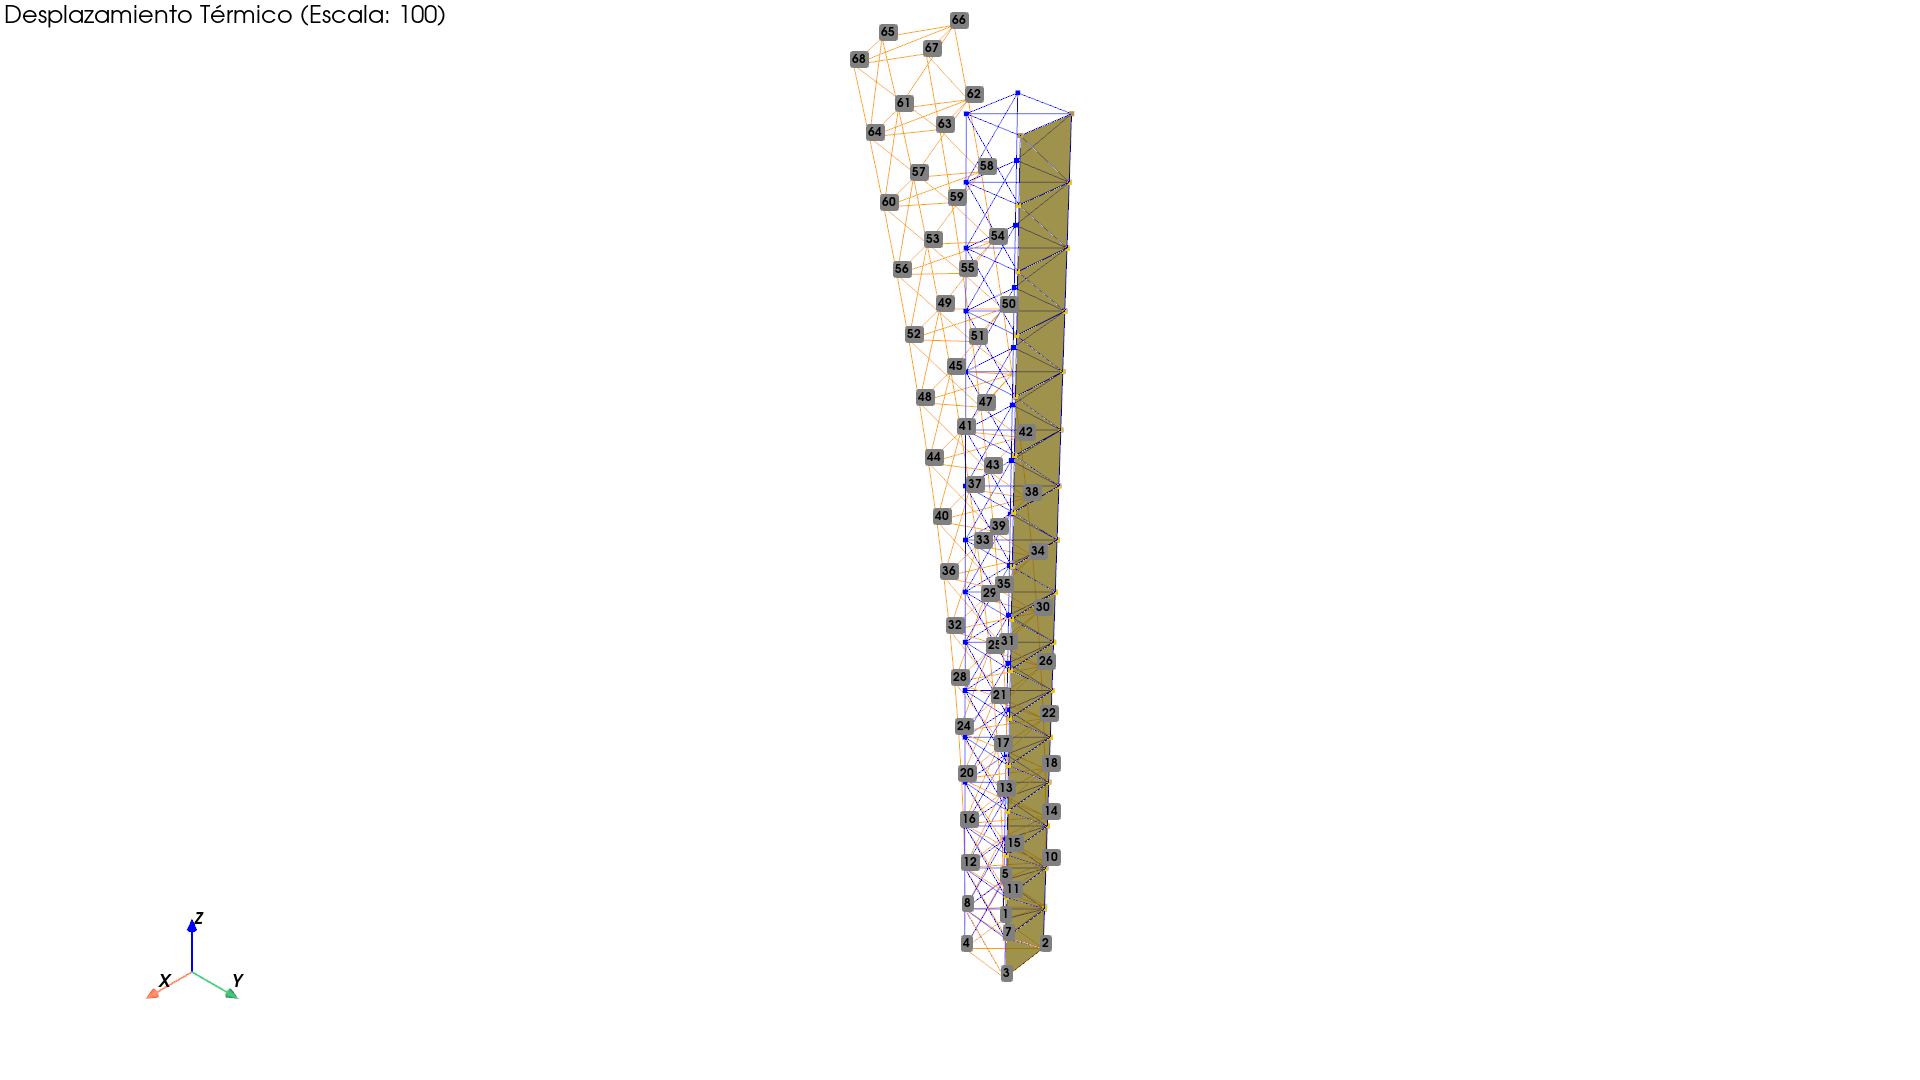
\includegraphics[width=\textwidth]{GRAFICOS/Desplazamientos Termicos False.png}
        \caption{Desplazamiento $\Delta T$ en estructura sin diagonales cruzadas.}
        \label{fig:imagen7}
    \end{minipage}
    \hfill
    \begin{minipage}{0.45\textwidth}
        \centering
        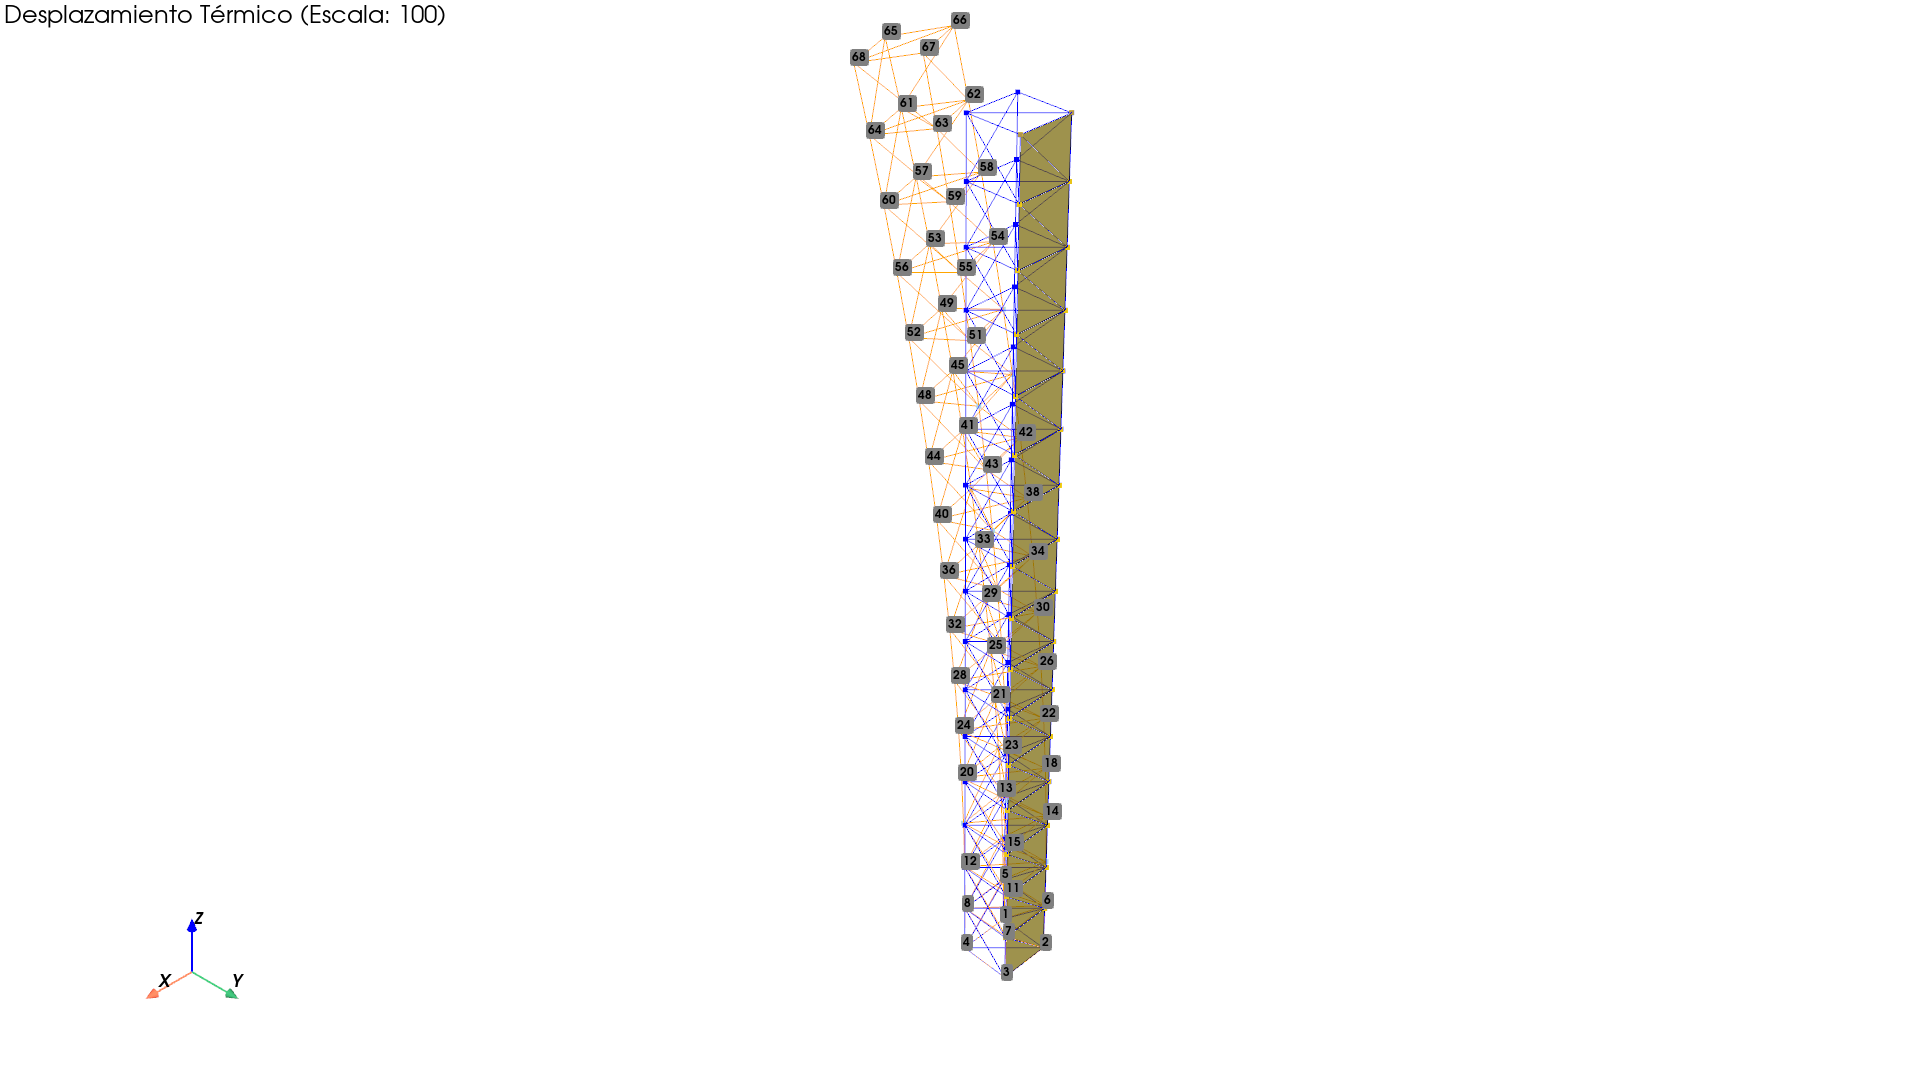
\includegraphics[width=\textwidth]{GRAFICOS/Desplazamientos Termicos True.png}
        \caption{Desplazamiento $\Delta T$ en estructura con diagonales cruzadas.}
        \label{fig:imagen8}
    \end{minipage}
\end{figure}

\begin{figure}[H]
    \centering
    \begin{minipage}{0.45\textwidth}
        \centering
        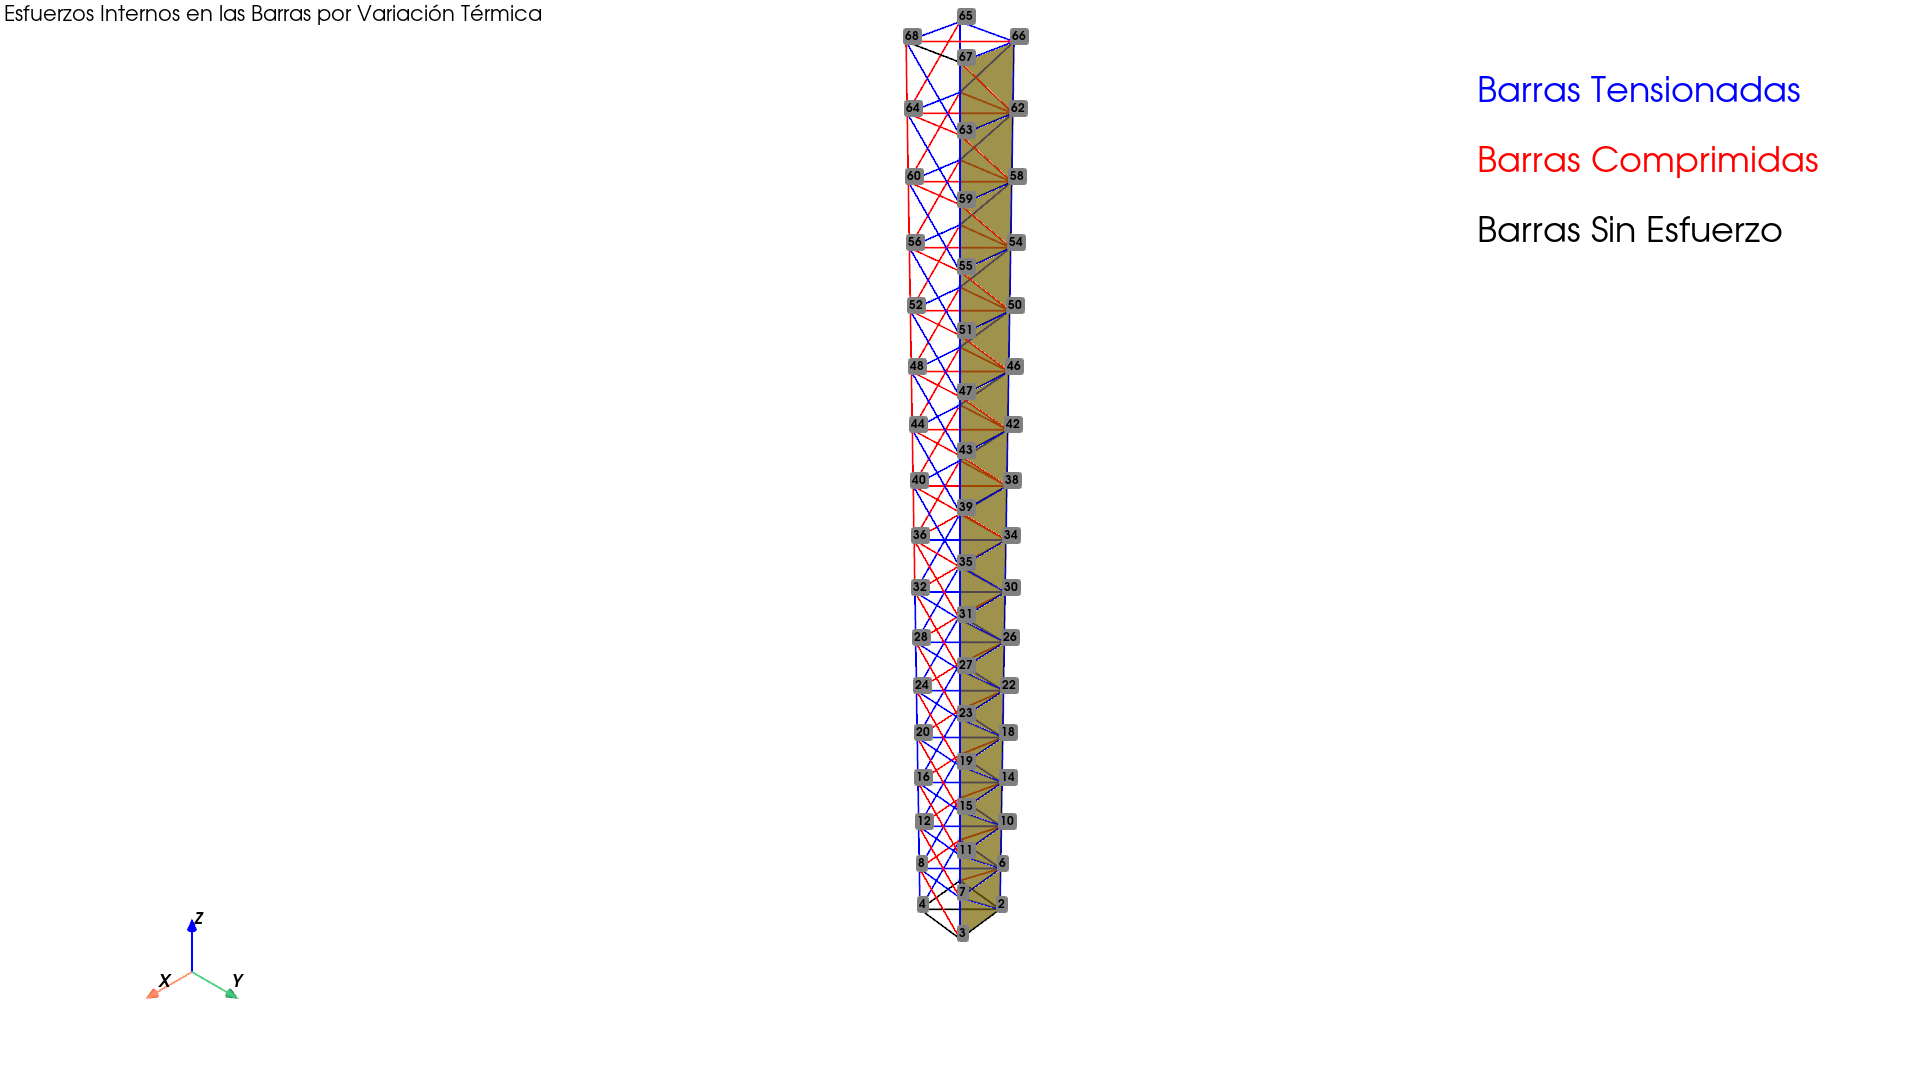
\includegraphics[width=\textwidth]{GRAFICOS/Esfuerzos Internos en las Barras por Variación Térmica False.png}
        \caption{Esfuerzos internos por $\Delta T$ en estructura sin diagonales cruzadas.}
        \label{fig:imagen77}
    \end{minipage}
    \hfill
    \begin{minipage}{0.45\textwidth}
        \centering
        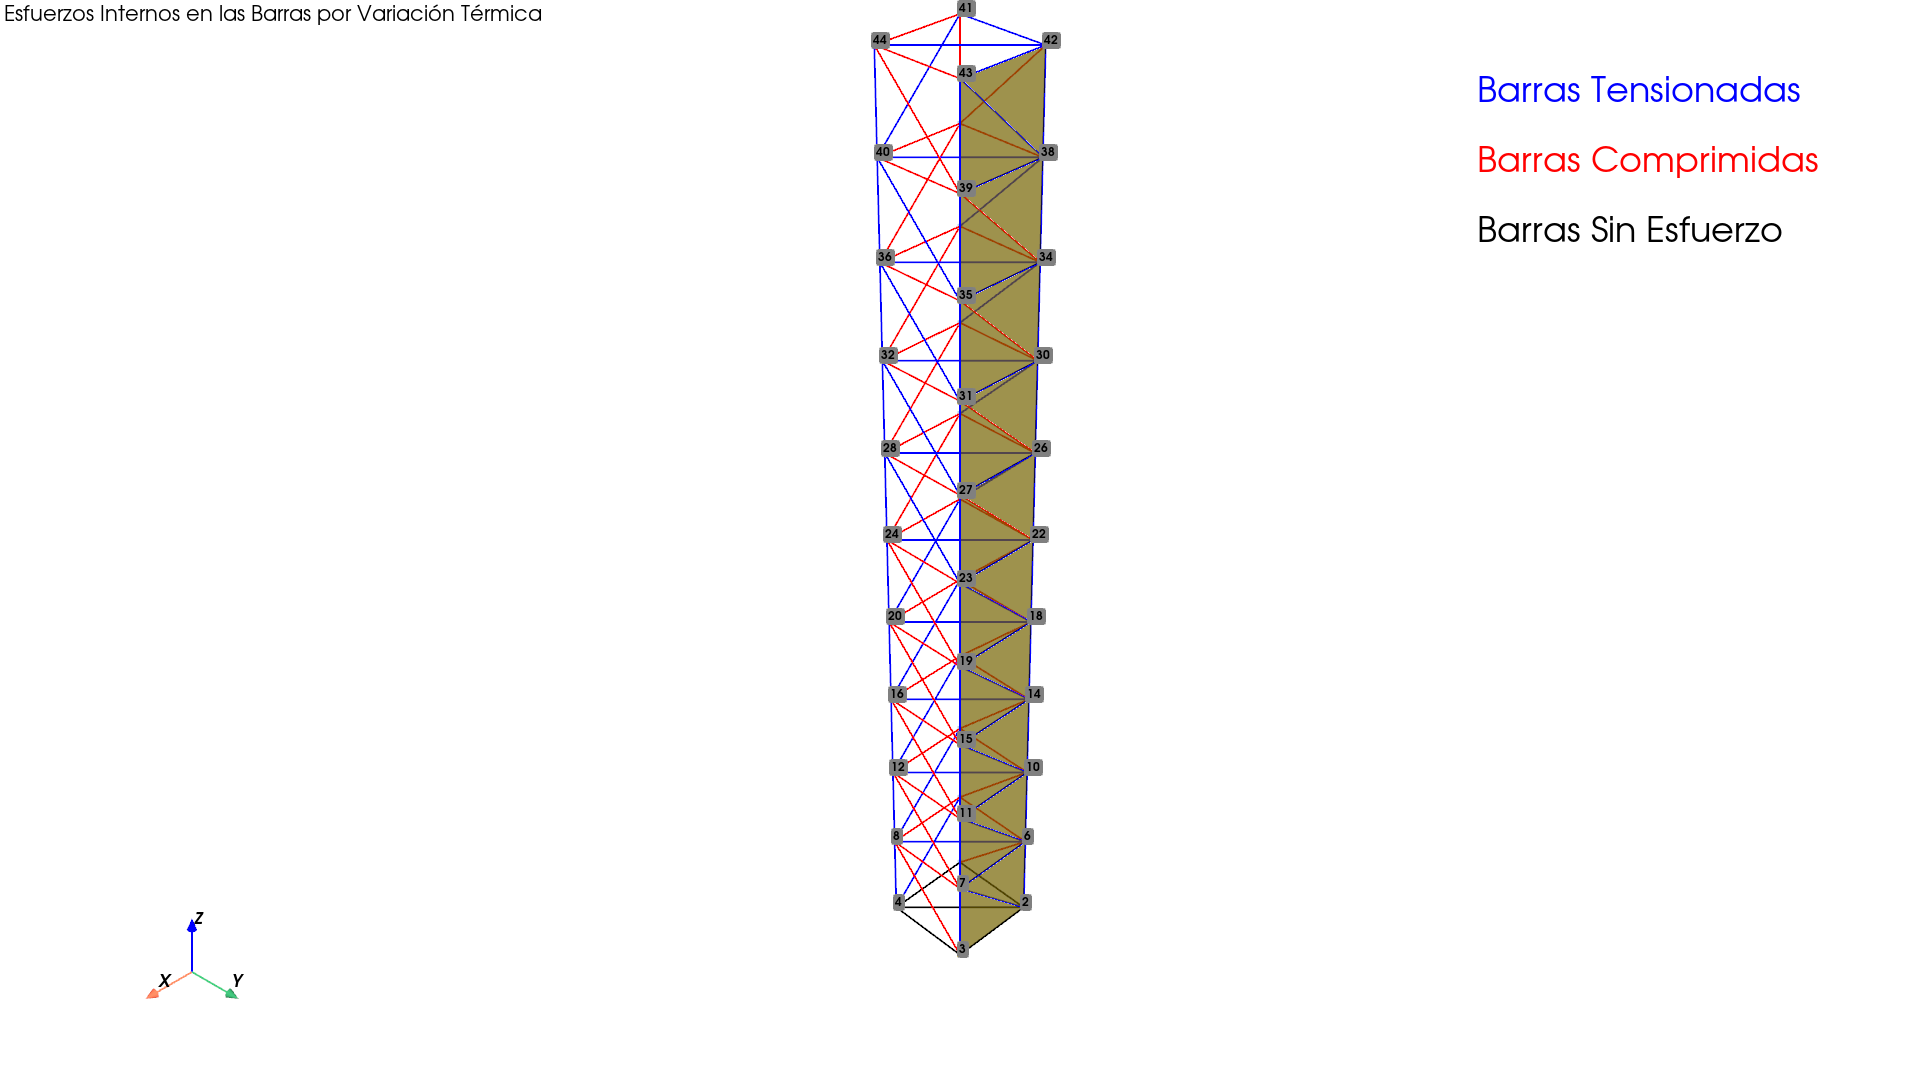
\includegraphics[width=\textwidth]{GRAFICOS/Esfuerzos Internos en las Barras por Variación Térmica True.png}
        \caption{Esfuerzos internos por $\Delta T$ en estructura con diagonales cruzadas.}
        \label{fig:imagen88}
    \end{minipage}
\end{figure}

Analizando y comparando cada imagen de deformaciones y tensiones en las direcciones X, Y, Z, se pueden obtener los siguientes resultados y observaciones.

En la imagen de desplazamiento inercial en la dirección X, la estructura muestra una deformación en la misma, desplazándose lateralmente.El mayor desplazamiento se observa en la parte superior, indicando que los elementos superiores son los más afectados frente a un cambio en su inercia. Los esfuerzos internos en las barras para esta dirección presentan barras comprimidas (de color rojo) en un lado y tensionadas (azules) en el lado opuesto, debido a la flexión inducida por la aceleración en X, las barras en diagonal muestran soportar los esfuerzos de tracción, mientras que la disposición cuadrada soporta los de compresión.

En la dirección Y, el comportamiento es similar al de la dirección X. Sin embargo, las barras en diagonal son las que soportan la mayor cantidad de esfuerzos de compresión, mientras que las cuadradas soportan los de tracción.

Por otro lado, la aceleración en Z provoca desplazamientos verticales en la estructura, con un patrón de deformación más simétrico en comparación con las direcciones X e Y. Los esfuerzos internos en las barras bajo aceleración en Z tienden a concentrarse de forma más uniforme en toda la estructura, debido a la acción directa de la gravedad. Esto hace que muchas barras experimenten compresión de manera más uniforme, y las tensiones máximas se distribuyan de forma homogénea a lo largo de la estructura.

En cuanto a la variación térmica, esta produce desplazamientos en toda la estructura sin una dirección específica, afectándola de manera global en lugar de inducir un desplazamiento en una sola dirección. Los esfuerzos internos en las barras se distribuyen en una forma variable, donde tanto barras diagonales como las cuadradas pueden soportar esfuerzos de tracción y compresión, lo que resulta en una combinación mas distribuida de esfuerzos internos.

\subsection{Parte 2}

En este caso se considerara que la aceleración del satélite de \(0.1 \, g\) puede ocurrir en cualquier dirección en el espacio 3D. Cada barra del reticulado tiene una "peor dirección" de aceleración, es decir, la dirección en la que se maximiza o minimiza su fuerza axial. El objetivo de esta sección es calcular las cargas axiales máximas y mínimas que cada barra debe resistir, considerando que la dirección de aceleración es arbitraria en tres dimensiones.

\subsubsection{Esfuerzos internos maximos de las barras}

\begin{figure}[H]
    \centering
    \includegraphics[width=0.7\textwidth]{GRAFICOS/Esfuerzos Internos Máximos en las Barras False False.png}
    \caption{Esfuerzos internos máximos en las barras.}
    \label{fig:imagen9}
\end{figure}

\begin{figure}[H]
    \centering
    \includegraphics[width=0.7\textwidth]{GRAFICOS/Esfuerzos Internos Máximos en las Barras True True.png}
    \caption{Esfuerzos internos máximos en las barras.}
    \label{fig:imagen99}
\end{figure}

En las figuras \ref{fig:imagen9} y \ref{fig:imagen99}, se observa que las tensiones más altas ocurren en las barras diagonales cercanas a los paneles, ya que estas barras soportan la mayor parte de la carga de la estructura. Las barras horizontales y verticales, por su parte, muestran tensiones más bajas, indicando que su función principal es estabilizar la estructura en lugar de soportar grandes fuerzas.

Las tensiones se ve que disminuyen a medida que se alejan de la estructura de anclaje, lo que sugiere que las cargas se distribuyen y se disipan a medida que se aleja de esta. Lo que podria sugerir que de ser necesario se deban reforzar las barras del comienzo de la estructura.
